% =============================================================================
% ch05_fusion.tex — Chapter 5: Sensor Fusion Architecture | Biomimetic Navigator
% =============================================================================

\selectlanguage{hebrew}
\section{ארכיטקטורת היתוך החישנים}
\label{sec:fusion}

\subsection{מבוא להיתוך בייזיאני}
היתוך חיישנים (\en{Sensor Fusion}) הוא התהליך של שילוב נתונים ממקורות שונים כדי להגיע להערכה מדויקת ואמינה יותר של מצב המערכת מאשר כל חיישן בנפרד. בבסיס התהליך עומד חוק בייס (\en{Bayes' Rule}), המאפשר לעדכן את ההסתברות של מצב $\mathbf{x}$ בהינתן תצפית $z$:
\begin{equation}
    p(\mathbf{x} | z_1, z_2) = \frac{p(z_1 | \mathbf{x}) p(z_2 | \mathbf{x}) p(\mathbf{x})}{p(z_1, z_2)}
    \label{eq:bayes_fusion}
\end{equation}

\subsection{מפת אמינות משוקללת}
במערכת ה-\en{NavigatorCrew}, אנו משתמשים במפת אמינות (\en{Confidence Map}) המשלבת את שלוש המודאליות. כל חיישן מקבל משקל $w_i$ בהתאם לתנאי הסביבה ולדיוקו היחסי באותו רגע.
\begin{equation}
    C_{\text{total}} = \sum_{i \in \{L, S, V\}} w_i \cdot C_i(x,y)
    \label{eq:weighted_sum}
\end{equation}
כאשר $L$ מסמל \en{LiDAR}, $S$ מסמל סונאר ו-$V$ מסמל \en{Vision}.

איור \ref{fig:sensor_fusion_heatmap} מציג סימולציה של מפת אמינות בסביבת חדר 10×10 מטרים:

\begin{figure}[H]
    \centering
    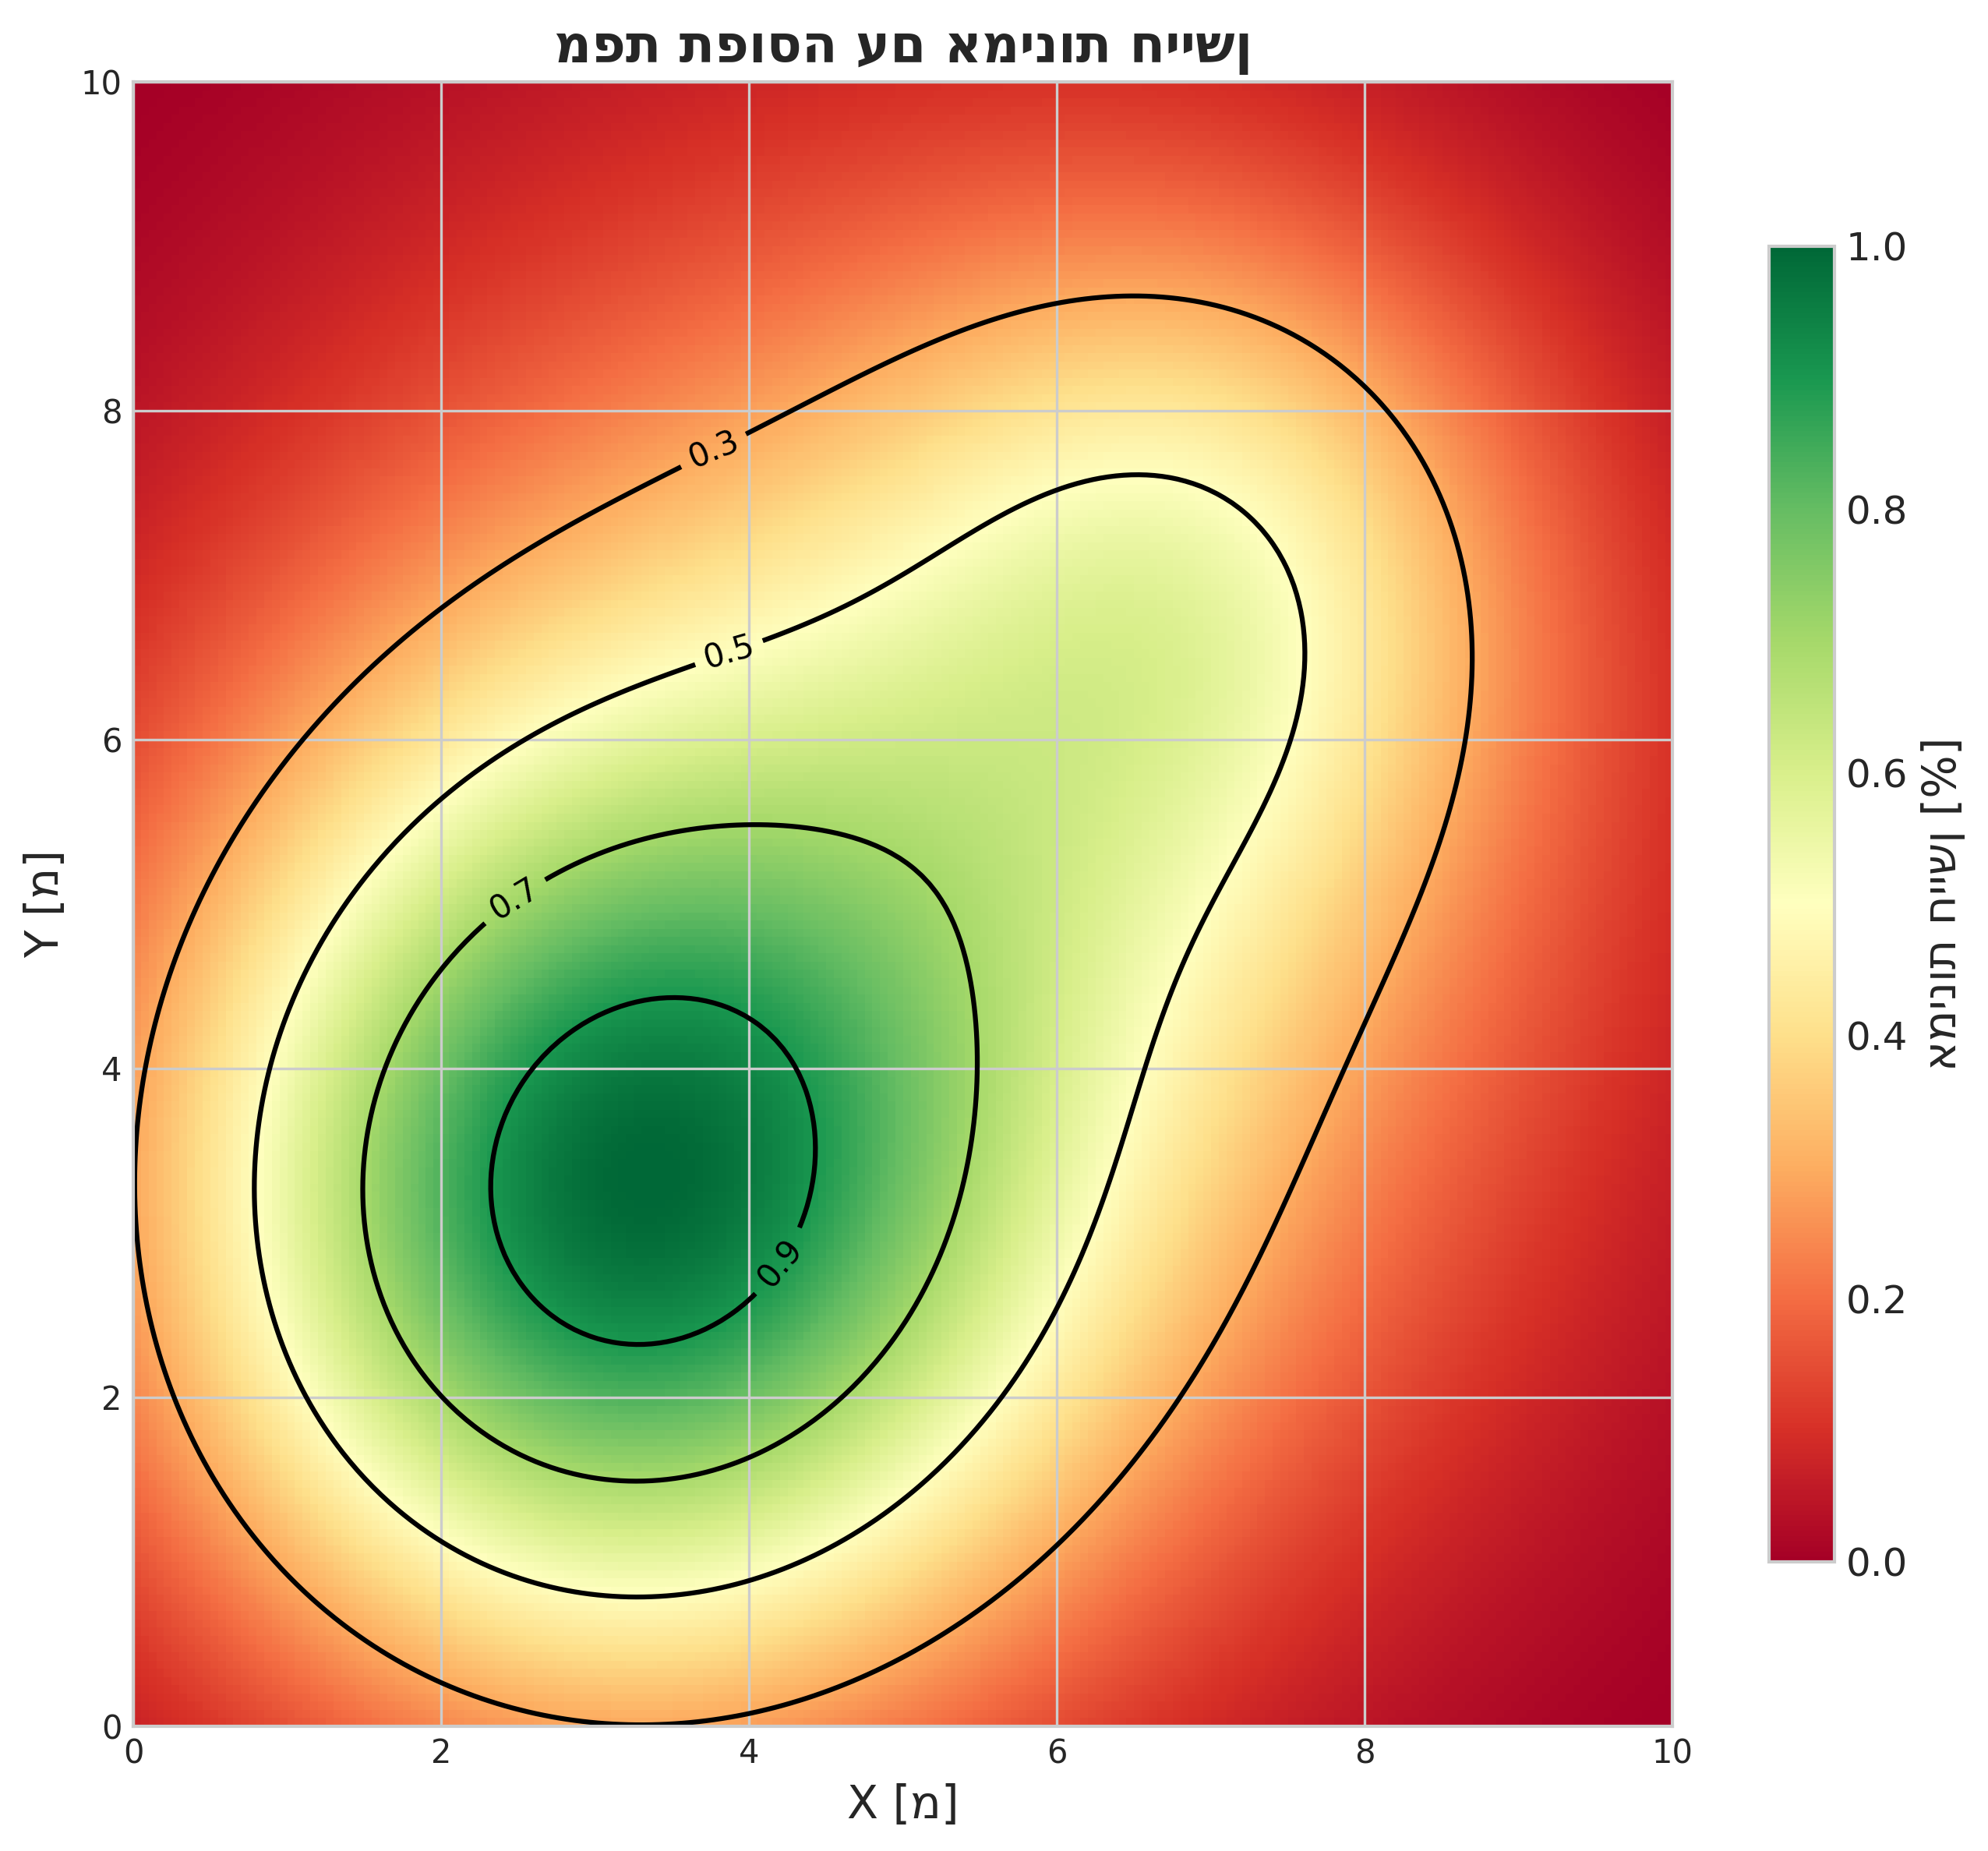
\includegraphics[width=0.8\columnwidth]{figures/fig_sensor_fusion_heatmap.png}
    \caption{מפת אמינות משוקללת של היתוך החיישנים. האזורים הירוקים מצביעים על רמת אמינות גבוהה בזיהוי מכשולים.}
    \label{fig:sensor_fusion_heatmap}
\end{figure}

\subsection{התמודדות עם קורלציה לא ידועה (\en{Covariance Intersection})}
אחת הבעיות המרכזיות בהיתוך חיישנים היא "ספירה כפולה" (\en{double counting}) של מידע כאשר מקורות הרעש של החיישנים מתואמים. כדי לפתור זאת, אנו משתמשים באלגוריתם \en{Covariance Intersection (CI)}, המבטיח הערכה שמרנית ובטוחה גם כאשר הקורלציה בין החיישנים אינה ידועה במדויק. \cite{Julier1997CovarianceIntersection}

\subsection{היתוך \en{EKF} מרובה-חיישנים}
במימוש שלנו, מטריצת המדידה $H$ ומטריצת הרעש $R$ מורחבות כדי להכיל את כל החיישנים בו-זמנית:
\begin{equation}
    R = \text{diag}(R_{\text{LiDAR}}, R_{\text{sonar}}, R_{\text{vision}})
    \label{eq:multi_sensor_r}
\end{equation}
זה מאפשר למסנן קלמן לעדכן את המצב בצורה אופטימלית תוך התחשבות באי-הוודאות הספציפית של כל חיישן ברגע נתון.
